\section*{Autores}
%Lembrar de reiniciar os contadores de autores aqui com o comando abaixo \setcounter{contador}{0}
\setcounter{contador}{0}

\begin{wrapfigure}{l}{0.17\textwidth}
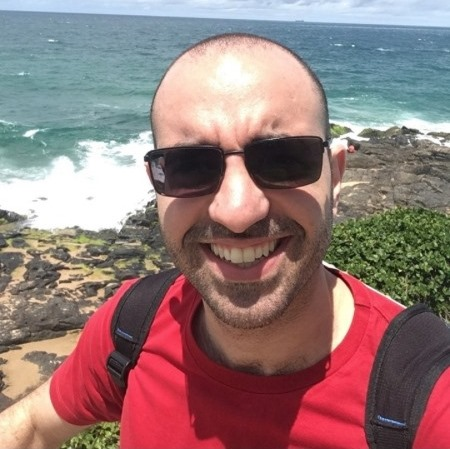
\includegraphics[trim= 0 2 0 0,clip,width=0.16\textwidth]{figuras/autor1.jpg}
\end{wrapfigure}

    \textbf{Dario Mendoza\textsuperscript{\contAutor}} Ingeniero en Mecatrónica graduado en - Universidad de las Fuerzas Armadas ESPE. Doutorando em Computação Aplicada pelo INPE - Instituto Nacional de Pesquisas Espaciais, na área de Engenharia de Software realizando estudos sobre metadados através da análise estática de código fonte e MSR (Mining Software Repositories). Mestre em Ciência da Computação(2016) pela UNIFEI - Universidade Federal de Itajubá. Engenheiro de Telecomunicações(2011) pelo INATEL - Instituto Nacional de Telecomunicações.  Técnico em Telecomunicações(2006) pela Escola Técnica de Eletrônica - ETE "FMC". É professor auxiliar do INATEL, atuando nos cursos de Engenharia da Computação e Engenharia de Software. Tem interesse nas áreas de Engenharia de Software Empírica e Desenvolvimento de Jogos\newline
    
\begin{wrapfigure}{l}{0.15\textwidth}
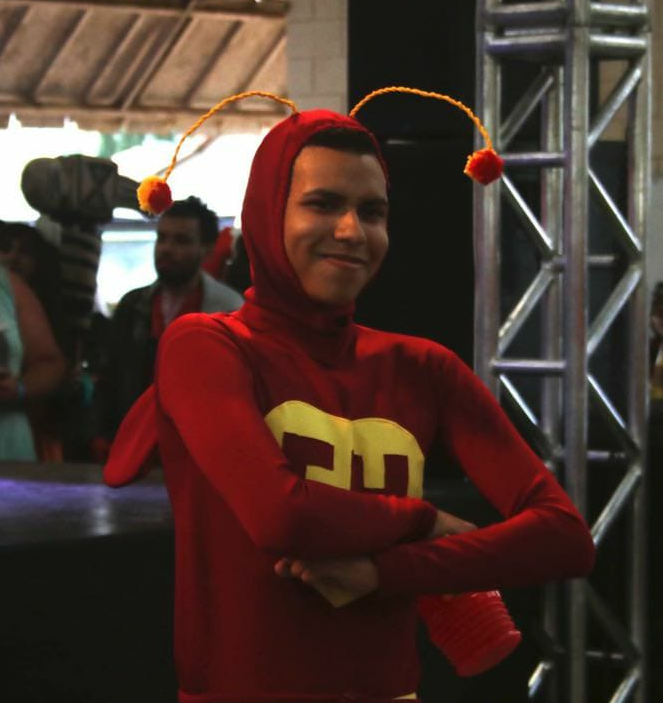
\includegraphics[trim= 0 2 0 0,clip,width=0.14\textwidth]{figuras/autor2.png}  
\end{wrapfigure}

   \textbf{Fernando Recalde\textsuperscript{\contAutor}} Ingeniero  graduado en - Universidad de las Fuerzas Armadas ESPE.é graduando em Tecnologia em Gestão de Telecomunicações pelo INATEL - Instituto Nacional de Telecomunicações. Tem interesse nas áreas de tecnologia, gestão e engenharia de produção.\newline

\begin{wrapfigure}{l}{0.15\textwidth}
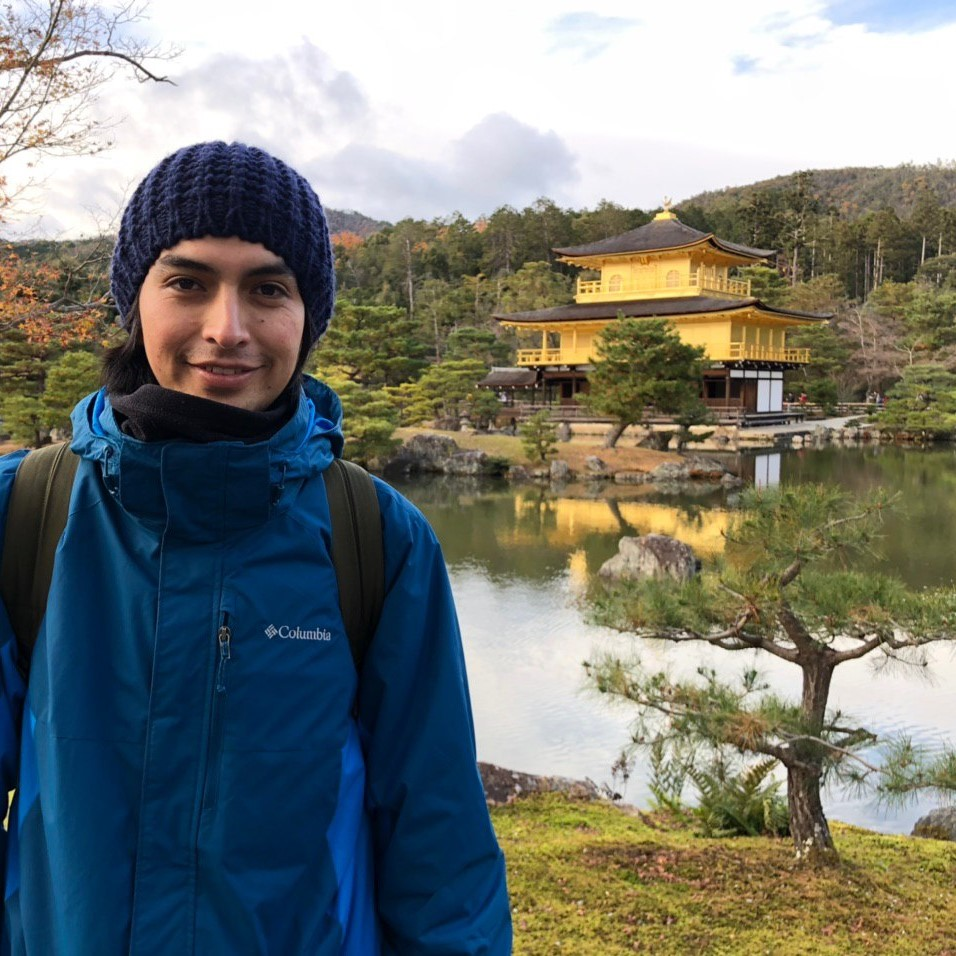
\includegraphics[trim= 0 2 0 0,clip,width=0.14\textwidth]{figuras/autor3.jpg}  
\end{wrapfigure}

   \textbf{Marcelo Ortiz\textsuperscript{\contAutor}} Ingeniero  en Mecatrónica graduado en - Universidad de las Fuerzas Armadas ESPE.\newline
   
\begin{wrapfigure}{l}{0.15\textwidth}
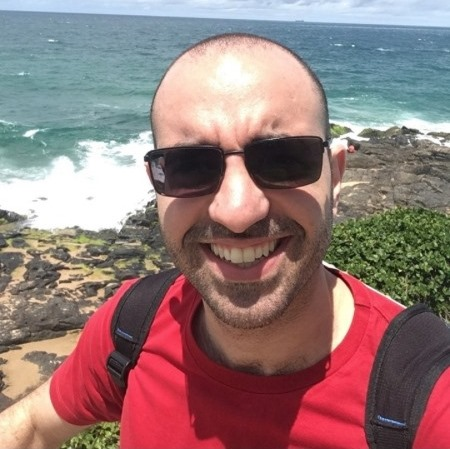
\includegraphics[trim= 0 2 0 0,clip,width=0.14\textwidth]{figuras/autor1.jpg}  
\end{wrapfigure}

   \textbf{Christopher Obando\textsuperscript{\contAutor}} Ingeniero  graduado en - Universidad de las Fuerzas Armadas ESPE.é graduando em Tecnologia em Gestão de Telecomunicações pelo INATEL - Instituto Nacional de Telecomunicações. Tem interesse nas áreas de tecnologia, gestão e engenharia de produção.